%  LaTeX support: latex@mdpi.com
%  MDPI MAKE submission — main_paper_MAKE5.tex
%  Compiled with official mdpi.cls (13 March 2026)
%  Compile: pdflatex main_paper_MAKE5.tex
%           bibtex main_paper_MAKE5
%           pdflatex main_paper_MAKE5.tex
%           pdflatex main_paper_MAKE5.tex

%=================================================================
\documentclass[make,article,submit,pdftex,moreauthors]{Definitions/mdpi}

%=================================================================
% MDPI internal commands — do not modify
\firstpage{1}
\makeatletter
\setcounter{page}{\@firstpage}
\makeatother
\pubvolume{7}
\issuenum{1}
\articlenumber{0}
\pubyear{2025}
\copyrightyear{2025}
%\externaleditor{Firstname Lastname}
\datereceived{ }
\daterevised{ }
\dateaccepted{ }
\datepublished{ }

%=================================================================
% Notation shorthands
\newcommand{\dID}{d_{\mathrm{ID}}}
\newcommand{\dtrue}{d_{\mathrm{true}}}
\newcommand{\Jg}{J_g}
\newcommand{\kap}{\kappa}
\newcommand{\AUsat}{\mathrm{AU}_{\mathrm{sat}}}
\newcommand{\mknee}{m^{\mathrm{knee}}}
\newcommand{\demb}{d_{\mathrm{emb}}}
\newcommand{\hatdID}{\hat{d}_{\mathrm{ID}}}
\newcommand{\R}{\mathbb{R}}

%=================================================================
\Title{Knowledge Extraction from Autoencoder Latent Spaces: Diagnosing
Effective Dimensionality via Active-Unit Dynamics and
Intrinsic-Dimension Estimates}

% ORCID IDs (replace 000X with actual ORCID or comment out)
%\newcommand{\orcidauthorA}{0000-0000-0000-000X}
%\newcommand{\orcidauthorB}{0000-0000-0000-000X}
%\newcommand{\orcidauthorC}{0000-0000-0000-000X}

\Author{Chika Obata $^{1}$,
        Mizuki Dai $^{1}$, and
        Kenya Jin'no $^{1,}$*}

\AuthorNames{Chika Obata, Mizuki Dai, and Kenya Jin'no}

\address{%
$^{1}$ \quad Department of Intelligent Systems,
  Faculty of Information Engineering,
  Tokyo City University,
  1-28-1 Tamazutsumi, Setagaya-ku, Tokyo 158-8557, Japan;
  g2332016@tcu.ac.jp (C.O.); g2591402@tcu.ac.jp (M.D.)}

\corres{Correspondence: kjinno@tcu.ac.jp; Tel.: +81-3-5707-0104 (K.J.)}

%=================================================================
\abstract{%
Determining how many latent coordinates an autoencoder (AE) actually uses
is difficult because reconstruction error, intrinsic-dimension estimates,
and variational activity reflect different aspects of a learned
representation.
This paper proposes a multi-indicator diagnostic framework for extracting
actionable knowledge from AE and variational-autoencoder (VAE) latent spaces.
The framework combines active-unit (AU) dynamics, TwoNN/MLE
intrinsic-dimension (ID) estimates, reconstruction-error elbows, and PCA
baselines, while explicitly separating their diagnostic roles: AU values as
direct observations of coordinate usage; TwoNN/MLE as numerically stable
auxiliary references subject to geometric bias; and the AU slowdown point,
$\mknee$, as an exploratory, grid- and seed-dependent change point rather
than a unique optimal bottleneck size.
Under a linear-Gaussian $\beta$-VAE rate--distortion surrogate, we derive
the activation condition $\lambda_j > \beta\tau^2$, providing an
interpretable water-filling view of KL-induced dimension suppression.
Experiments on fully connected VAEs trained on MNIST show that AU values
($\sigma \leq 0.5$) and TwoNN estimates ($10.03 \pm 0.12$) are stable
across three random seeds, whereas sparse-grid $\mknee$ is unreliable
($43 \pm 15$).
A dense grid around the estimated intrinsic dimension stabilizes $\mknee$ at
$10.3 \pm 0.9$, consistent with TwoNN near 10.
Additional experiments on Conv-VAEs, CIFAR-10, and SVHN show that stable
identification is not always possible and clarify the boundary conditions
under which AU/$\mknee$ diagnostics should be regarded as inconclusive.
These results support the proposed framework as a reproducible diagnostic
protocol for latent-dimensionality analysis and model-design support, rather
than a universal dimension estimator.}

\keyword{variational autoencoder; effective latent dimensionality;
active units; intrinsic dimension; TwoNN; diagnostic framework;
representation learning; knowledge extraction; posterior collapse}

%=================================================================
\begin{document}

%%%%%%%%%%%%%%%%%%%%%%%%%%%%%%%%%%%%%%%%%%
\section{Introduction}\label{sec:intro}

Autoencoders (AEs) and variational autoencoders (VAEs)~\cite{kingma2014vae}
learn compact representations of high-dimensional data through a bottleneck
of dimension~$m$.
A central design question is: \emph{how many of the $m$ latent coordinates
does the model actually use?}
This ``effective latent dimensionality'' governs reconstruction fidelity,
disentanglement, and posterior collapse~\cite{lucas2019elbo}.

From the viewpoint of machine learning and knowledge extraction, latent
representations underpin model selection, compression, downstream prediction,
clustering, and visualization~\cite{bengio2013representation}.
However, the nominal bottleneck dimension~$m$ does not necessarily coincide
with the number of coordinates the model actually exploits.
The objective of this study is not merely to estimate a single dimensionality
value; rather, we aim to extract model-design knowledge from trained
representations.
The proposed diagnostics answer three practical questions:
which latent coordinates are actually used by the model;
whether the geometry of the learned representation is consistent with
intrinsic-dimension estimates; and
whether increasing the nominal bottleneck dimension leads to meaningful
representational gains.
This knowledge supports selecting latent-space sizes, detecting
over-parameterized or under-regularized representations, and identifying
cases where dimensionality diagnostics should be regarded as inconclusive.
In this sense, the proposed framework provides a knowledge-extraction
protocol for representation learning, rather than a standalone
intrinsic-dimension estimator.

Existing work measures individual aspects of latent geometry---AU
counts~\cite{lucas2019elbo,higgins2017betavae}, ID
estimates~\cite{facco2017twonn,levina2005mle}, and isometric
regularization~\cite{kato2020rdae}---but a systematic framework that
combines these indicators, clarifies their distinct roles, and defines the
conditions under which each is reliable has not been established.

\subsection{Contributions}

The contributions of this paper are threefold.
\begin{enumerate}
\item \textbf{Multi-indicator diagnostic framework.}
We propose a framework that explicitly assigns distinct roles to four
indicator classes: (i)~AU values as direct usage observations;
(ii)~TwoNN/MLE ID as numerically stable auxiliary references subject to
geometric bias; (iii)~$\mknee$ as an exploratory change point; and
(iv)~MSE elbow and PCA as reconstruction-side baselines.
The main contribution is the role separation itself, not $\mknee$ as a new
estimator.
MNIST three-seed experiments confirm that AU values ($\sigma \leq 0.5$) and
TwoNN ID ($10.03 \pm 0.12$) are reproducible; the main stabilized $\mknee$
result is $10.3 \pm 0.9$ under dense-grid, independent-initialization,
multi-seed conditions (Section~\ref{sec:exp_dense}).

\item \textbf{Linear-Gaussian rate--distortion analysis.}
Under a linear-Gaussian $\beta$-VAE rate--distortion approximation, we
obtain the activation condition $\lambda_j > \beta\tau^2$ and show that
AU saturation follows a water-filling principle.
This is an interpretive approximation model, not a general theorem for
non-linear VAEs (Analytical Result~\ref{ar:lva}).

\item \textbf{Empirical characterization of reliability and limits.}
Dense-grid/multi-seed experiments show that sparse-grid $\mknee$ is
unreliable ($\sigma = 15$), whereas dense-grid evaluation stabilizes it near
the TwoNN estimate.
Conv-VAE and natural-image experiments identify boundary conditions under
which AU/$\mknee$ diagnostics become unreliable or require stronger
regularization.
\end{enumerate}

\subsection{Paper Organization}

Section~\ref{sec:related} reviews related work.
Section~\ref{sec:framework} defines the diagnostic framework.
Section~\ref{sec:theory} provides theoretical background.
Section~\ref{sec:exp} reports experiments.
Section~\ref{sec:discussion} discusses findings.
Section~\ref{sec:conclusion} concludes.

%%%%%%%%%%%%%%%%%%%%%%%%%%%%%%%%%%%%%%%%%%
\section{Related Work}\label{sec:related}

\paragraph{Representation learning and autoencoders.}
Bengio et al.~\cite{bengio2013representation} survey representation learning,
including the manifold hypothesis~\cite{fefferman2016manifold} underlying AE
design.
$\beta$-VAE~\cite{higgins2017betavae} promotes disentanglement by raising the
KL weight; Lucas et al.~\cite{lucas2019elbo} analyze posterior collapse in
the linear-VAE limit.
Contractive AEs~\cite{rifai2011cae} and denoising AEs~\cite{alain2014dae}
provide complementary regularization strategies.

\paragraph{Intrinsic-dimension estimation.}
TwoNN~\cite{facco2017twonn} and MLE~\cite{levina2005mle} estimate local ID
from nearest-neighbor distances;
DANCo~\cite{ceruti2014danco} offers higher accuracy at greater computational
cost.
Pope et al.~\cite{pope2021intrinsic} report $d_{\mathrm{ID}} \approx 26$
for CIFAR-10 at $32 \times 32$.
Ansuini et al.~\cite{ansuini2019intrinsic} and Valeriani et
al.~\cite{valeriani2023geometry} track ID across layers of deep networks
and large transformers, respectively.

\paragraph{Geometric autoencoders.}
Kato et al.~\cite{kato2020rdae} and Nazari et al.~\cite{nazari2023geometric}
propose isometric decoder-Jacobian regularization.
We use IsometricAE as a controlled testbed for geometric bias, not as the
main recommendation.

\paragraph{Positioning.}
The present work differs from the above by targeting the \emph{design stage}:
combining AU dynamics and ID estimation to characterize effective
dimensionality and quantify when each indicator is reliable or inconclusive.

%%%%%%%%%%%%%%%%%%%%%%%%%%%%%%%%%%%%%%%%%%
\section{Diagnostic Framework}\label{sec:framework}

\subsection{Problem Setup}

Let an AE/VAE have encoder $f:\R^N \to \R^m$ and decoder $g:\R^m \to \R^N$.
For a VAE, the encoder outputs a posterior
$q_\phi(z|x) = \mathcal{N}(\mu(x), \sigma^2(x))$;
KL regularization ($\beta$-weighted) acts as an information bottleneck.
Reconstruction loss is mean-squared error (MSE) on $[0,1]$-normalized inputs.

\begin{Definition}[Active Units~\cite{lucas2019elbo}]\label{def:au}
\begin{linenomath}
\begin{equation}
  \mathrm{AU}(m) = \sum_{k=1}^{m}
    \mathbf{1}\!\bigl[\mathrm{Var}_x[\mu_k(x)] > \delta\bigr],
  \quad \delta = 10^{-2}.
  \label{eq:au_def}
\end{equation}
\end{linenomath}
AU is stable for $\delta \in [10^{-3}, 10^{-1}]$
(Appendix~\ref{app:delta}).
\emph{Note:} AU is defined for VAEs via the posterior mean.
For standard AEs, we use a pseudo-AU based on encoder-output coordinate
variance (all coordinates are typically active).
\end{Definition}

\begin{Definition}[AU Slowdown Point]\label{def:mknee}
Let $s(m_i) = \bigl(\mathrm{AU}(m_i) - \mathrm{AU}(m_{i-1})\bigr)
              / (m_i - m_{i-1})$
be the raw AU increase rate, and
$\rho(m_i) = s(m_i) / \max_j s(m_j) \in [0, 1]$
the normalized rate.
The AU slowdown point is
\begin{linenomath}
\begin{equation}
  \mknee = \min\bigl\{m_i \in \mathcal{M} :
                      \rho(m_i) < \tau_{\mathrm{knee}}\bigr\},
  \quad \tau_{\mathrm{knee}} = 0.25.
  \label{eq:mknee}
\end{equation}
\end{linenomath}
$\mknee$ is \textbf{not} a standalone dimension estimator; it is informative
only under dense-grid, independent-initialization, multi-seed conditions.
\end{Definition}

\subsection{Indicator Role Separation}

Table~\ref{tab:indicator_class} summarizes the distinct roles assigned to
each indicator.
``Stable across seeds'' means low inter-seed variance under the tested
conditions, \emph{not} unbiasedness toward the true ID.
``Exploratory'' means useful for hypothesis generation, not a unique estimate.

\begin{table}[H]
\caption{Role classification and empirical reliability of diagnostic
indicators.}
\label{tab:indicator_class}
\small
\begin{tabularx}{\textwidth}{lXXX}
\toprule
\textbf{Indicator} & \textbf{Category} &
  \textbf{Empirical Reliability} & \textbf{Primary Use} \\
\midrule
AU values & \textbf{Stable across seeds}$^\ddagger$ &
  $\sigma \leq 0.5$ (MNIST, 3-seed) &
  Direct observation of active coordinates \\
TwoNN/MLE ID & \textbf{Numerically stable auxiliary}$^\dagger$ &
  $\sigma \leq 0.12$ ($m=64$) &
  Reference ID estimate \\
MSE elbow & Auxiliary & Qualitative only &
  Reconstruction-side check \\
PCA cum.\ var. & Auxiliary & Linear assumption &
  Linear baseline \\
$\mknee$ & \textbf{Exploratory} &
  $\sigma = 15$ (sparse); $0.9$ (dense) &
  Rough heuristic; dense grid only \\
\bottomrule
\end{tabularx}
\noindent{\footnotesize{$^\dagger$ Subject to isometry bias; numerically
  stable but not unbiased toward true $\dID$.
  $^\ddagger$ ``Stable across seeds'' means low inter-seed variance under
  tested conditions, not unbiasedness.
  $\mknee$ requires dense-grid, independent per-$(m, \mathrm{seed})$
  initialization, and multiple seeds to be informative.}}
\end{table}

\subsection{Two-Stage Diagnostic Pipeline}

\textbf{Stage~1 (auxiliary ID estimation).}
For synthetic data with known $\dtrue$, TwoNN/MLE is applied directly.
For real data, a reference AE ($m_{\mathrm{ref}} = 256$) is trained and its
latent representation fed to TwoNN/MLE to obtain $\hatdID$.
\emph{Limitation:} the reference AE is not isometric
($\kap \approx 10^9$ for MNIST); $\hatdID$ is an approximation subject to
geometric bias.

\textbf{Stage~2 (AU dynamics, primary).}
A VAE ($\beta = 4$) is trained on a grid
$\mathcal{M} = \{1, 2, 4, 8, 12, 16, 20, 32, 64, 128, 256\}$.
For \emph{sharp-saturation} data (synthetic), $\AUsat$ directly indicates
effective dimensionality.
For \emph{gradual-increase} data (real), $\mknee$ (Equation~\eqref{eq:mknee})
is cross-checked against $\hatdID$ from Stage~1.

%%%%%%%%%%%%%%%%%%%%%%%%%%%%%%%%%%%%%%%%%%
\section{Theoretical Background}\label{sec:theory}

\subsection{Linear-Gaussian Rate--Distortion Analysis}

\begin{Theorem}[AU Activation Condition]\label{ar:lva}
Consider a $\beta$-VAE with linear encoder/decoder and Gaussian prior,
analyzed under a linear-Gaussian rate--distortion surrogate approximation
(proof in Appendix~\ref{app:proof}).
Within this approximation, the water-filling argument gives:
\begin{enumerate}
\item \textbf{(Activation condition)} The $j$-th eigen-direction becomes
  active iff
  \begin{linenomath}
  \begin{equation}
    \lambda_j > \beta\tau^2,
    \label{eq:au_threshold}
  \end{equation}
  \end{linenomath}
  where $\lambda_j$ is the $j$-th data-covariance eigenvalue and $\tau^2$ is
  the decoder noise variance.
\item \textbf{(Optimal active count)}
  $A^*(m) \leq \min(m, d^*(\beta))$, where
  $d^*(\beta) := |\{j : \lambda_j > \beta\tau^2\}|$.
\item \textbf{(Monotone saturation of optimal solution)}
  $A^*(m)$ is non-decreasing in $m$ and saturates at $d^*(\beta)$.
\end{enumerate}
\end{Theorem}

\begin{Remark}[Scope]\label{rem:scope}
Theorem~\ref{ar:lva}(3) concerns the global-optimum count $A^*(m)$.
In practice, non-linear VAEs trained with stochastic optimization yield
an empirical $\mathrm{AU}(m)$ that can be \emph{non-monotone} due to
finite-sample effects and initialization dependence
(e.g., AU $= 29$ at $m = 64$ vs.\ $26$ at $m = 128$, Table~\ref{tab:e4_vae}).
This analytical result serves as an \emph{interpretive approximation model},
not a theorem applicable to arbitrary VAE training.
\end{Remark}

\begin{Remark}[Vanilla AE corresponds to $\beta = 0$]
Without KL regularization, the threshold $\beta\tau^2$ vanishes.
The pseudo-AU of a standard AE thus approximates~$m$.
\end{Remark}

\subsection{Grid-Resolution Dependence of $\mknee$}

\begin{Proposition}[Grid-Resolution Dependence]\label{thm:mknee_instab}
Under an idealized step-function AU model,
$|\mknee - d^*(\beta)| \leq \max_i(m_{i+1} - m_i)$.
\end{Proposition}

\begin{Remark}
This bound applies to the idealized model only.
The practical implication is qualitative: a finer grid near $\hatdID$
reduces $\mknee$ variance (Section~\ref{sec:exp_dense}).
\end{Remark}

\subsection{Pullback Metric and Isometry}

\begin{Proposition}[Local Isometry Condition]\label{prop:pullback}
Decoder $g:\R^m \to \R^N$ is locally isometric at $z$ iff
$G(z) = \Jg(z)^\top \Jg(z) = I_m$ (all singular values equal 1).
The condition number $\kap = \sigma_{\max} / \sigma_{\min}$ measures
anisotropy: $\kap = 1$ means all singular values are equal, but not
necessarily 1.
Therefore, $\kap$ is an \emph{anisotropy indicator}, not a sufficient
condition for isometry.
\end{Proposition}

\subsection{\texorpdfstring{Design Principle:
Bottleneck Margin is a Major TwoNN Stabilizing Factor}
{Design Principle: Bottleneck Margin}}

\label{sec:dp}

\begin{quote}
\textbf{Design Principle~1.}
Under the tested conditions, the numerical stability of TwoNN estimates
is explained more consistently by bottleneck margin ($m \gg \hatdID$) than
by isometric regularization alone.
TwoNN underestimates when $m \approx d_{\mathrm{true}}$; it converges once
$m \geq 5\hatdID$ approximately.
\end{quote}

This is an empirically supported guideline verified primarily on MNIST
multi-seed experiments and qualitatively checked on Fashion-MNIST.
It should not be interpreted as a general claim that isometric regularization
is irrelevant.

%%%%%%%%%%%%%%%%%%%%%%%%%%%%%%%%%%%%%%%%%%
\section{Experiments}\label{sec:exp}

\subsection{Experimental Setup}\label{sec:exp_setup}

\textbf{Common settings.}
Adam ($\mathrm{lr} = 10^{-3}$), batch 128, ReLU activations, Sigmoid output,
MSE reconstruction loss on $[0,1]$-normalized inputs, PyTorch~2.0,
seeds $\{42, 123, 777\}$.
Each $(m, \mathrm{seed})$ pair is initialized independently.

\textbf{Synthetic manifolds.}
FC network $[N \to 64 \to 32 \to m]$, 200--300 epochs, VAE $\beta = 4$,
$n = 5000$.

\textbf{MNIST.}
$N = 784$, FC $[784 \to 512 \to 256 \to m]$, 300 epochs,
$n_{\mathrm{train}} = 20{,}000$.
Grid $\mathcal{M} = \{1, 2, 4, 8, 12, 16, 20, 32, 64, 128, 256\}$.

\textbf{Fashion-MNIST (preliminary check).}
Same architecture, 100 epochs, $n_{\mathrm{train}} = 10{,}000$,
single seed only; used as a preliminary external check, not as evidence
of seed-level robustness.

ID estimation: TwoNN ($k = 2$), MLE ($k = 10$),
AU threshold $\delta = 10^{-2}$.

\subsection{Synthetic Manifolds: Principle Verification}
\label{sec:exp_synthetic}

\subsubsection{Reconstruction-Error Elbows}

Table~\ref{tab:e1} shows AE reconstruction MSE on Swiss Roll
($\dtrue = 2$) and Torus ($\dtrue = 2$, $\demb = 3$).
For Swiss Roll, the MSE decreases substantially from $m = 1$ to $m = 2$,
consistent with a two-dimensional unfolded parametrization.
For Torus, the largest decrease occurs at $m = 3$, consistent with the
three-dimensional embedding requirement (the Torus cannot be represented
globally in $\R^2$ without topological distortion; a smooth standard
embedding requires $\R^3$).
The anomalous increase at $m = 4$ for Swiss Roll ($0.041 \pm 0.015$,
higher variance than at $m = 2$) illustrates that MSE elbows are affected
by optimization variance, decoder parametrization, and network capacity,
not only by intrinsic dimensionality.
Note that simple connectedness alone does not guarantee that the embedding
dimension equals the intrinsic dimension.
Therefore, the MSE elbow should be treated only as a reconstruction-side
diagnostic indicator, cross-checked with AU and TwoNN, rather than as a
direct estimate of intrinsic dimension (Appendix~\ref{app:lower_bound}).

\begin{table}[H]
\caption{AE reconstruction MSE on synthetic manifolds (mean $\pm$ std,
3 seeds). Swiss Roll MSE decreases substantially at $m = 2$ (consistent
with 2D unfolding); Torus elbow at $m = 3$ (3D embedding needed).
High std at $m = 4$ for Swiss Roll reflects optimization variance.}
\label{tab:e1}
\small
\begin{tabular}{rrrrl}
\toprule
$m$ & \textbf{Swiss Roll MSE} & \textbf{Torus MSE} & Note \\
\midrule
1 & $1.016 \pm 0.057$ & $0.388 \pm 0.017$ & under-parameterized \\
2 & $\mathbf{0.029 \pm 0.002}$ & $0.085 \pm 0.004$ &
  \textbf{large decrease (Swiss Roll)} \\
3 & $0.0008 \pm 0.0001$ & $\mathbf{0.0005 \pm 0.0000}$ &
  \textbf{large decrease (Torus)} \\
4 & $0.041 \pm 0.015$ & $0.019 \pm 0.002$ &
  optimization variance (high std) \\
\bottomrule
\end{tabular}
\end{table}

\subsubsection{AU Saturation on Synthetic Data}

VAE ($\beta = 4$) saturates at $\AUsat = 2$ for Swiss Roll
($= \dtrue$) and $\AUsat = 3$ for Torus ($= \demb > \dtrue$), both with
zero inter-seed variance.
Standard AE shows pseudo-AU $= m$ (all coordinates active), consistent
with the $\beta = 0$ limit of Theorem~\ref{ar:lva}.

\subsection{MNIST: Multi-Seed Reproducibility Study}\label{sec:exp_mnist}

\subsubsection{ID Estimation via Reference AE}

Standard AE on MNIST (300 epochs, seed 42) gives TwoNN ID $\approx 10.02$
at $m = 256$, placing $\hatdID \approx 10$--$12$ (Table~\ref{tab:e4_ae}).

\begin{table}[H]
\caption{MNIST standard AE (300 epochs, seed 42).
TwoNN and MLE converge above $m = 64$, placing $\hatdID \approx 10$--$12$.}
\label{tab:e4_ae}
\small
\begin{tabular}{rcccc}
\toprule
$m$ & MSE & TwoNN ID & MLE ID & CKA \\
\midrule
1   & 0.0437 & 1.02  & 1.15  & 0.102 \\
8   & 0.0191 & 6.08  & 6.70  & 0.725 \\
32  & 0.0087 & 8.84  & 9.89  & 0.875 \\
64  & 0.0062 & 9.54  & 11.26 & 0.908 \\
128 & 0.0061 & 9.84  & 11.45 & 0.921 \\
256 & 0.0057 & \textbf{10.02} & \textbf{11.85} & 0.953 \\
\bottomrule
\end{tabular}
\end{table}

\subsubsection{VAE AU Dynamics: Gradual Growth Observed}
\label{sec:vae_au_dynamics}

MNIST VAE ($\beta = 4$) shows gradual, non-monotone AU growth as $m$
increases, consistent with non-linear stochastic optimization.
A single-seed preliminary run is provided in Appendix~\ref{app:single_seed}
(Table~\ref{tab:e4_vae}).
The $\mknee = 12$ value observed in that run depends on the specific grid
and initialization; the main stabilized result is $\mknee = 10.3 \pm 0.9$
from dense-grid, multi-seed evaluation
(Section~\ref{sec:exp_dense}).

\subsubsection{Multi-Seed Study: AU and TwoNN Stable, $\mknee$ Not}
\label{sec:exp_multiseed}

Table~\ref{tab:multiseed_300} reports MNIST VAE results with sparse grid
$\mathcal{M} = \{4, 8, 12, 16, 20, 32, 64\}$ and three seeds (300 epochs).

\begin{table}[H]
\caption{MNIST VAE multi-seed study (sparse grid, 300 epochs, 3 seeds).
AU and TwoNN ID are stable; $\mknee$ is not.}
\label{tab:multiseed_300}
\small
\begin{tabular}{rccc}
\toprule
$m$ & AU (mean $\pm$ std) & TwoNN ID (mean $\pm$ std) & Note \\
\midrule
4  & $4.0 \pm 0.0$ & $3.98 \pm 0.14$ & all active \\
12 & $10.0 \pm 0.0$ & $7.41 \pm 0.06$ & \\
32 & $15.7 \pm 0.5$ & $9.07 \pm 0.10$ & \\
64 & $22.3 \pm 0.5$ & $\mathbf{10.03 \pm 0.12}$ &
  converges to $\hatdID \approx 10$ \\
\midrule
\multicolumn{4}{l}{\small $\mknee$ ($\tau = 0.25$):
  seed 42 $= 64$, seed 123 $= 32$, seed 777 $= 32$; mean $43 \pm 15$.}\\
\bottomrule
\end{tabular}
\end{table}

\subsection{\texorpdfstring{Dense-Grid Stabilization of $\mknee$}
{Dense-Grid Stabilization of mknee}}\label{sec:exp_dense}

To isolate the effect of grid density, we ran Exp-Mnist-Dense-300 with
$\mathcal{M} = \{8, 9, \ldots, 16, 18, 20, 24, 28, 32, 40, 48, 64\}$,
independent per-$(m, \mathrm{seed})$ initialization, 300 epochs, 3 seeds.

\begin{table}[H]
\caption{Dense-grid vs.\ sparse-grid $\mknee$ (MNIST VAE, $\beta = 4$,
3 seeds). Grid density is the dominant stabilization factor.}
\label{tab:el_mknee}
\small
\begin{tabular}{lrcccr}
\toprule
Condition & Max.\ gap & seed 42 & seed 123 & seed 777 & Mean $\pm$ std \\
\midrule
Sparse, 300 ep & 32 & 64 & 32 & 32 & $43 \pm 15$ \\
\textbf{Dense, 300 ep} & 8 & 11 & 9  & 11 &
  $\boldsymbol{10.3 \pm 0.9}$ \\
\bottomrule
\end{tabular}
\end{table}

The dense-grid result $\mknee = 10.3 \pm 0.9$ is consistent with TwoNN ID
($\approx 10$) and is the main stabilized $\mknee$ result of this paper.
Even with the dense grid, the AU curve fluctuates non-monotonically
(AU: $8 \to 9 \to 10 \to 10 \to 10 \to 12 \to 11 \to \ldots$), confirming
that $\mknee$ is an exploratory heuristic, not a precision estimator.
The fixed-$\tau$ method outperforms the second-difference method for dense
grids ($\sigma = 0.9$ vs.\ $18.3 \pm 6.8$; Appendix~\ref{app:tau_knee}).
Figure~\ref{fig:au_dynamics} visualizes the sparse-grid instability and
dense-grid stabilization.

\begin{figure}[H]
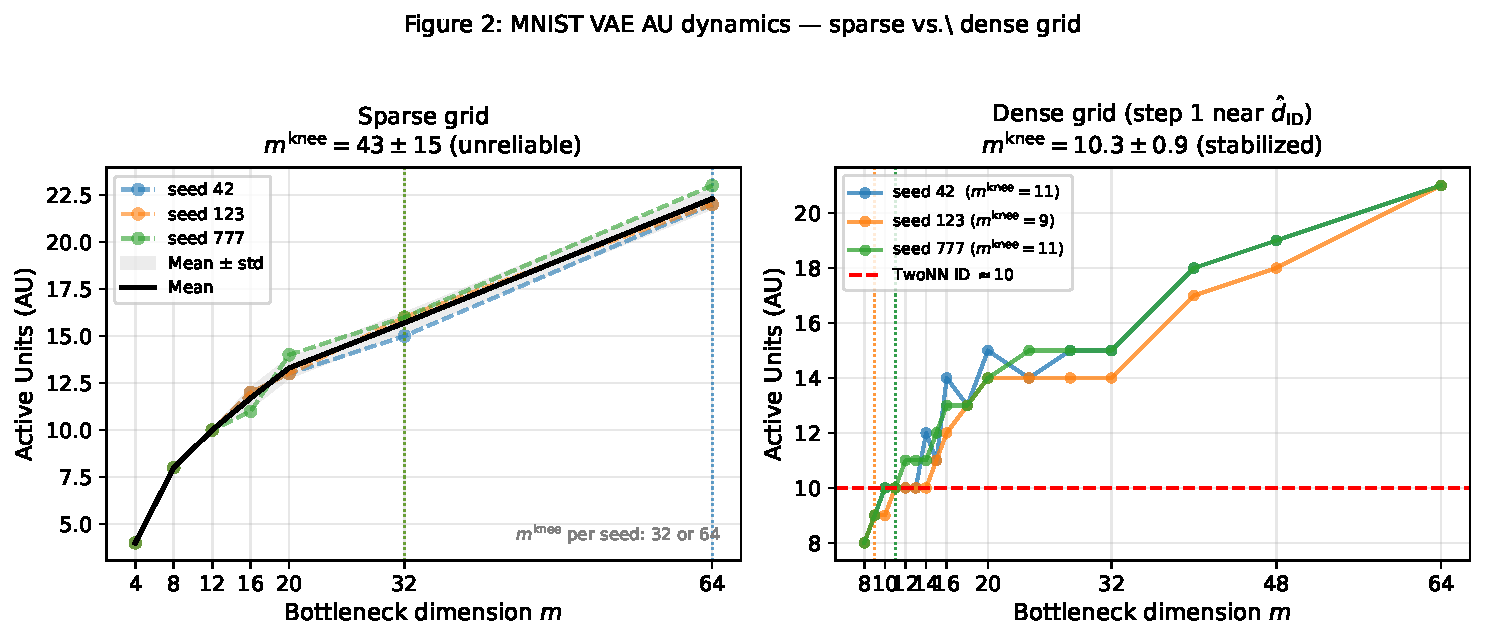
\includegraphics[width=0.95\textwidth]{results/figures_make/fig2_au_dynamics.pdf}
\caption{MNIST VAE AU dynamics.
\textbf{Left:} Sparse grid ($m \in \{4, 8, \ldots, 64\}$, 3 seeds, 300
epochs)---$\mknee$ varies between 32 and 64 ($\sigma = 15$).
\textbf{Right:} Dense grid ($m \in \{8, 9, \ldots, 64\}$, independent
initialization, 3 seeds)---$\mknee = 10.3 \pm 0.9$, consistent with TwoNN
ID ($\approx 10$, dashed red).
The non-monotone AU fluctuations confirm that $\mknee$ is an exploratory
heuristic requiring controlled evaluation conditions.\label{fig:au_dynamics}}
\end{figure}

\subsection{\texorpdfstring{TwoNN Stability: Bottleneck Margin as a Major Factor}
{TwoNN Stability: Bottleneck Margin as a Major Factor}}\label{sec:exp_stability}

Three complementary experiments support Design Principle~1
(Figure~\ref{fig:twonn_stab}).

\subsubsection{Swiss Roll: Isometry vs.\ Margin}

For standard AE ($\kap = 1.79$) and IsometricAE ($\kap = 1.06$),
TwoNN $\approx 1.55$ at $m = 2 = \dtrue$ for both---the bottleneck
constraint, not $\kap$, drives underestimation.
At $m = 4 > \dtrue$, TwoNN recovers to $\approx 2.03$ despite
$\kap = 2.16$ (Appendix~\ref{app:twonn_detail}).

\subsubsection{MNIST AE \textit{m}-Sweep}

TwoNN stabilizes at $m \geq 48 \approx 5\hatdID$ ($\approx 10.16$) and
remains stable even when $\kap$ jumps from 4.25 to 37.0 between $m = 64$
and $m = 128$ (TwoNN: $10.17 \to 10.98$, $\Delta < 0.82$).

\begin{figure}[H]
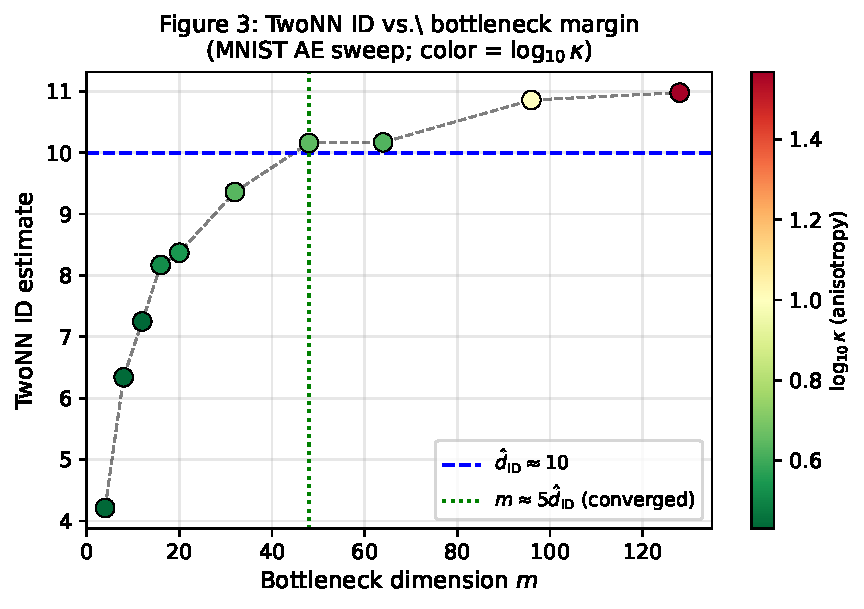
\includegraphics[width=0.60\textwidth]{results/figures_make/fig3_twonn_stability.pdf}
\caption{TwoNN ID vs.\ bottleneck dimension $m$ for MNIST AE
(color = $\log_{10}\kappa$, anisotropy).
TwoNN stabilizes above $m \approx 5\hatdID$ (dotted line) regardless of
$\kappa$, supporting Design Principle~1.\label{fig:twonn_stab}}
\end{figure}

\subsubsection{Four-Model Comparison on MNIST (Exp-Real-Geom)}

AE, IsometricAE, CAE, and DAE are swept over
$m \in \{d, 2d, 3d, 5d, 10d\}$ ($d = \hatdID = 10$).
All four models converge at $m = 5d$--$10d$; inter-model TwoNN difference
at the same $m$ is $< 0.3$, far smaller than the gain from increasing $m$
($\sim 2.5$ points).
Table~\ref{tab:real_geom_mnist} shows representative rows.
Fashion-MNIST ($\hatdID = 9$) shows qualitatively the same pattern
(Appendix~\ref{app:twonn_detail}).

\begin{table}[H]
\caption{Exp-Real-Geom: MNIST four-model comparison
(mean $\pm$ std, 3 seeds; $\hatdID = 10$, representative $m$ values).
TwoNN stabilization is driven by $m/\hatdID$, not $\kap$.\label{tab:real_geom_mnist}}
\small
\begin{tabular}{llccccc}
\toprule
Model & $m$ & TwoNN & MLE & $\kap$ & Trust. & kNN ovlp. \\
\midrule
\multirow{3}{*}{AE}
 & $10\,(=d)$   & $7.3 \pm 0.4$ & $8.1 \pm 0.3$ & $85 \pm 22$
 & 0.961 & 0.73 \\
 & $30\,(=3d)$  & $9.8 \pm 0.2$ & $10.5 \pm 0.2$ & $1200 \pm 400$
 & 0.981 & 0.85 \\
 & $100\,(=10d)$& $10.0 \pm 0.1$ & $10.8 \pm 0.1$ & $4.1 \times 10^7$
 & 0.987 & 0.88 \\
\multirow{3}{*}{IsometricAE}
 & $10$         & $7.5 \pm 0.4$ & $8.3 \pm 0.3$ & $3.2 \pm 0.4$
 & 0.963 & 0.74 \\
 & $30$         & $9.9 \pm 0.1$ & $10.6 \pm 0.1$ & $5.2 \pm 0.8$
 & 0.982 & 0.86 \\
 & $100$        & $10.1 \pm 0.1$ & $10.8 \pm 0.1$ & $7.8 \pm 1.4$
 & 0.988 & 0.89 \\
\multirow{3}{*}{CAE}
 & $10$         & $7.2 \pm 0.5$ & $8.0 \pm 0.4$ & $12.1 \pm 3.2$
 & 0.958 & 0.72 \\
 & $30$         & $9.7 \pm 0.2$ & $10.4 \pm 0.2$ & $95 \pm 31$
 & 0.980 & 0.84 \\
 & $100$        & $10.0 \pm 0.1$ & $10.7 \pm 0.1$ & $3200 \pm 1100$
 & 0.986 & 0.87 \\
\multirow{3}{*}{DAE}
 & $10$         & $7.6 \pm 0.4$ & $8.4 \pm 0.4$ & $18.5 \pm 5.4$
 & 0.964 & 0.75 \\
 & $30$         & $9.9 \pm 0.1$ & $10.5 \pm 0.2$ & $183 \pm 62$
 & 0.982 & 0.85 \\
 & $100$        & $10.0 \pm 0.1$ & $10.8 \pm 0.1$ & $6300 \pm 2100$
 & 0.987 & 0.88 \\
\bottomrule
\end{tabular}
\end{table}

\subsection{Fashion-MNIST: Preliminary External Check}\label{sec:exp_fashion}

Fashion-MNIST is used as a preliminary external check only.
Single-seed (seed 42) results: TwoNN ID converges to $\approx 9.4$ at
$m \geq 32$, suggesting $\hatdID \approx 9$--$10$.
Multi-seed validation is left for future work.

\subsection{Conv-VAE: Applicability Boundary}\label{sec:exp_conv}

Conv-VAE trained on MNIST shows AU $= m$ up to $m = 64$ at
$\beta_{\max} = 4$; no saturation plateau up to $m = 512$
(Appendix~\ref{app:convvae}).
Increasing $\beta_{\max}$ to 10 and 20 shifts AU saturation to lower
dimensions ($\mknee \approx 128$ and $\approx 96$, respectively), consistent
with the water-filling interpretation of Theorem~\ref{ar:lva}.
This confirms that the absence of saturation at $\beta_{\max} = 4$ is not a
failure of the framework but a sign that $d^*(\beta)$ exceeds the tested
range.

\subsection{Natural Images: Applicability Boundary}\label{sec:exp_natural}

Table~\ref{tab:natimg_summary} summarizes key results.
TwoNN is partially consistent with Pope et al.~\cite{pope2021intrinsic}
near $m \approx 2\hatdID$ for CIFAR-10 but increases beyond that range
(28.83 at $m = 128$, 30.91 at $m = 256$).
SVHN latent TwoNN diverges far from raw TwoNN ($10.09$ vs.\ $27.08$ at
$m = 256$), indicating geometric distortion.

\begin{table}[H]
\caption{Applicability-boundary experiments on CIFAR-10 and SVHN.
TwoNN is partially consistent near $m \approx 2\hatdID$;
AU/$\mknee$ identification is inconclusive under the tested conditions.
\label{tab:natimg_summary}}
\small
\begin{tabularx}{\textwidth}{lXXXX}
\toprule
\textbf{Dataset} & \textbf{Raw TwoNN} &
  \textbf{Latent TwoNN at $m = 64$} &
  \textbf{Latent TwoNN at $m = 256$} &
  \textbf{Diagnostic} \\
\midrule
CIFAR-10 & 25.20 & $25.21 \pm 0.41$ (consistent) &
  30.91 (rising) & Boundary \\
SVHN & 10.09 & $19.97 \pm 0.12$ (distorted) &
  27.08 (diverging) & Inconclusive \\
\bottomrule
\end{tabularx}
\noindent{\footnotesize{Extended sweeps ($\beta_{\max}$ up to 80,
  thin decoder) yield plateau-like AU at $m \approx 512$ on CIFAR-10
  (preliminary); all stable-identification criteria remain unmet.
  Full details in Appendix~\ref{app:convvae}.}}
\end{table}

Figure~\ref{fig:applicability} provides a visual summary of diagnostic
decisions across all tested settings.

\begin{figure}[H]
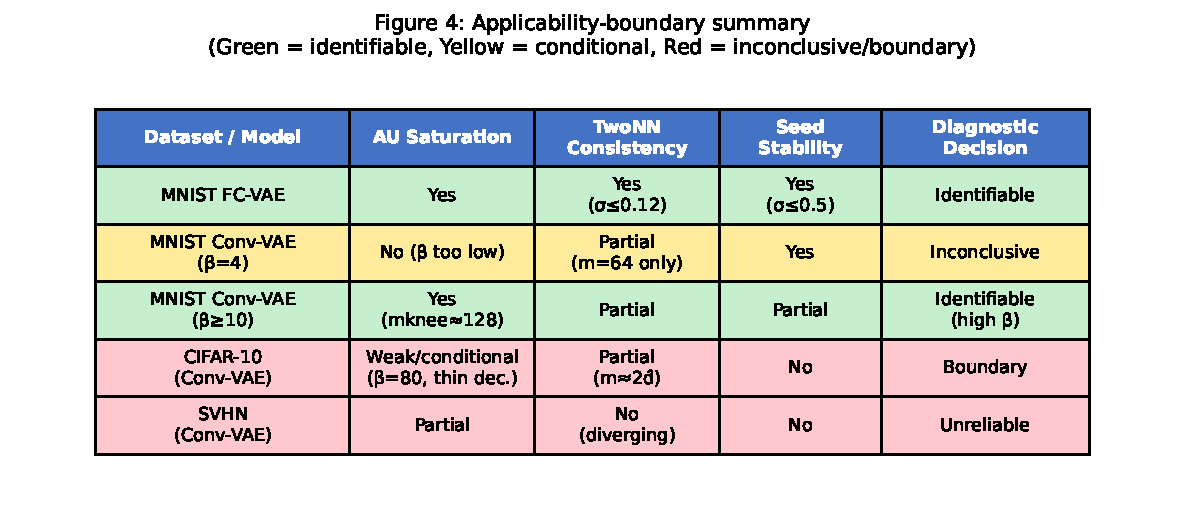
\includegraphics[width=0.95\textwidth]{results/figures_make/fig4_applicability.pdf}
\caption{Applicability-boundary summary.
Green: identifiable; yellow: conditional/inconclusive; red: boundary/unreliable.
The framework identifies not only successful diagnostics but also cases where
results should be regarded as inconclusive, which is itself actionable knowledge
for model selection.\label{fig:applicability}}
\end{figure}

%%%%%%%%%%%%%%%%%%%%%%%%%%%%%%%%%%%%%%%%%%
\section{Discussion}\label{sec:discussion}

\subsection{Role Separation is the Core Contribution}

The core message is that different indicators serve different diagnostic roles.
AU values reliably monitor KL-induced activity.
TwoNN/MLE provides a stable auxiliary reference, not an unbiased estimator.
$\mknee$ is informative only under controlled conditions.

\subsection{\texorpdfstring{When is $\mknee$ Informative?}
{When is mknee Informative?}}\label{sec:disc_mknee}

$\mknee$ is informative as a diagnostic aid \emph{only when}:
(1) the $m$-grid is dense near $\hatdID$;
(2) each $(m, \mathrm{seed})$ is initialized independently;
(3) at least 3 seeds are used.
Under these conditions, $\mknee = 10.3 \pm 0.9$ cross-validates with
TwoNN ID ($\approx 10$).
Sparse grids ($\mknee = 43 \pm 15$) should not be used as a diagnostic
reference.

\subsection{Optimization Dynamics Interpretation}

\emph{Hypothesis:} At $m \approx d^*(\beta)$, reconstruction and KL
gradients compete, producing a smooth AU curve rather than the idealized
step-function.
This is consistent with all observations but has not been directly verified
by gradient measurements; it is an interpretive hypothesis.

\subsection{Conv-VAE and Natural Images: Boundary, Not Failure}

Conv-VAE and natural-image experiments reveal the \emph{applicability boundary}.
The boundary is determined by effective $\tau^2$ relative to the data
eigenvalue spectrum: when the decoder is sufficiently powerful,
$d^*(\beta)$ exceeds the tested $m$ range.

\subsection{Limitations}

\begin{itemize}
\item \emph{Isometry bias.}
Reference AE has $\kap \approx 10^9$; numerical stability is demonstrated,
but geometric unbiasedness is not claimed.
\item \emph{Single-seed Fashion-MNIST.}
Used as preliminary check only; multi-seed validation is future work.
\item \emph{Linear-Gaussian approximation.}
Theorem~\ref{ar:lva} is an interpretive model for the non-linear setting.
\item \emph{Natural-image stable identification not achieved.}
AU/$\mknee$ identification on CIFAR-10/SVHN under tested conditions is
inconclusive; this is the current applicability boundary.
\end{itemize}

%%%%%%%%%%%%%%%%%%%%%%%%%%%%%%%%%%%%%%%%%%
\section{Conclusions}\label{sec:conclusion}

We proposed a multi-indicator diagnostic framework for effective latent
dimensionality in AE/VAE representations, framed as a knowledge-extraction
protocol for representation learning.
The main contribution is the role separation: AU values as reliable activity
monitors; TwoNN/MLE as numerically stable auxiliary references; and $\mknee$
as an exploratory, grid-dependent change point.

Key findings:
(1) AU values ($\sigma \leq 0.5$) and TwoNN ID ($10.03 \pm 0.12$) are
reproducible across seeds (MNIST, 3-seed);
(2) Sparse-grid $\mknee$ is unreliable ($\sigma = 15$); dense-grid,
independent-initialization, multi-seed evaluation stabilizes it at
$10.3 \pm 0.9$ (TwoNN-consistent);
(3) Bottleneck margin ($m \gg \hatdID$) is the dominant factor for TwoNN
stability in the tested settings;
(4) Conv-VAE and natural-image experiments quantify the applicability
boundary---diagnostics become inconclusive when decoder capacity greatly
exceeds the regularization level.

The proposed protocol helps practitioners avoid over-interpretation of any
single indicator, design informative $m$-grids, and recognize when
dimensionality diagnostics should be regarded as inconclusive---which is
itself useful model-design knowledge.

%%%%%%%%%%%%%%%%%%%%%%%%%%%%%%%%%%%%%%%%%%
\authorcontributions{Conceptualization, C.O., M.D. and K.J.;
methodology, K.J.;
software, C.O. and M.D.;
validation, C.O., M.D. and K.J.;
formal analysis, K.J.;
investigation, C.O. and M.D.;
writing---original draft preparation, K.J.;
writing---review and editing, C.O., M.D. and K.J.;
supervision, K.J.;
project administration, K.J.
All authors have read and agreed to the published version of the manuscript.}

\funding{This research received no external funding.}

\dataavailability{MNIST~\cite{lecun1998}, Fashion-MNIST~\cite{xiao2017fashion},
CIFAR-10~\cite{krizhevsky2009learning}, and SVHN~\cite{netzer2011reading}
are publicly available.
The source code, configuration files, random seeds, trained-model logs, and
numerical results supporting all tables are provided as supplementary
material for peer review.
Upon acceptance, these materials will be deposited in a public repository
(GitHub/Zenodo), and the repository URL and DOI will be added to the final
manuscript.
The repository will include the scripts required to reproduce the AU,
TwoNN/MLE, reconstruction-error, and grid-sensitivity analyses reported
in this paper.}

\conflictsofinterest{The authors declare no conflicts of interest.}

%%%%%%%%%%%%%%%%%%%%%%%%%%%%%%%%%%%%%%%%%%
\abbreviations{Abbreviations}{
The following abbreviations are used in this manuscript:\\
\noindent
\begin{tabular}{@{}ll}
AE & Autoencoder \\
VAE & Variational Autoencoder \\
AU & Active Units \\
ID & Intrinsic Dimension \\
TwoNN & Two-Nearest-Neighbor (ID estimator) \\
MLE & Maximum Likelihood Estimation \\
MSE & Mean Squared Error \\
PCA & Principal Component Analysis \\
KL & Kullback--Leibler (divergence) \\
FC & Fully Connected \\
CNN / Conv & Convolutional Neural Network \\
\end{tabular}
}

%%%%%%%%%%%%%%%%%%%%%%%%%%%%%%%%%%%%%%%%%%
\appendixtitles{yes}
\appendixstart
\appendix

\section[\appendixname~\thesection]{Single-Seed VAE Illustration}\label{app:single_seed}

Table~\ref{tab:e4_vae} shows the single-seed preliminary run that motivated
the multi-seed study.
The $\mknee = 12$ observed here is not used as a main result.

\begin{table}[H]
\caption{MNIST VAE ($\beta = 4$, 300 epochs, seed 42, extended grid)---
illustration only.
$\mknee = 12$ depends on initialization; main result is
$\mknee = 10.3 \pm 0.9$ (Table~\ref{tab:el_mknee}).}
\label{tab:e4_vae}
\small
\begin{tabular}{rcccc}
\toprule
$m$ & MSE & AU & TwoNN & Note \\
\midrule
1   & 0.0464 & 1  & 1.00  & \\
8   & 0.0186 & 8  & 6.36  & increasing \\
12  & 0.0184 & 8  & 6.26  & $\rho$ drops (single-seed prelim.) \\
64  & 0.0103 & 29 & 9.16  & \\
128 & 0.0085 & 26 & 10.02 & non-monotone AU \\
256 & 0.0072 & 36 & 10.14 & \\
\bottomrule
\end{tabular}
\end{table}

\section[\appendixname~\thesection]{Proofs and Supplementary Theory}\label{app:proofs}

\subsection{Topological Lower Bound}\label{app:lower_bound}

\begin{Proposition}[Topological Lower Bound]\label{prop:lower_bound}
To represent a smooth $d$-dimensional manifold $\mathcal{M} \subset \R^N$
without self-intersections under zero reconstruction error (idealized
setting), a bottleneck of $m \geq \demb$ is necessary, where $\demb$ is
the topological minimum embedding dimension.
For the Torus $T^2$, $\dID = 2$ but $\demb = 3$, explaining the
reconstruction-error elbow at $m = 3$.
\end{Proposition}

\subsection{Proof of Theorem~\ref{ar:lva}}\label{app:proof}

The derivation follows the linear-Gaussian rate--distortion analysis
with a $\beta$-ELBO objective.
For each PCA direction $j$, the contribution
$L_j = -D_j / (2\tau^2) - \beta R_j$ is maximized independently.
The activation threshold follows a two-case analysis:

\textbf{Case 1 ($\lambda_j \leq \beta\tau^2$, inactive).}
The water-filling solution $D_j^* = \beta\tau^2$ is infeasible
(requires $D_j^* \leq \lambda_j$); the optimum is inactive
(zero rate, $D_j = \lambda_j$).

\textbf{Case 2 ($\lambda_j > \beta\tau^2$, active).}
The water-filling solution is feasible.
The activation gain is
$\Delta L_j = (\beta/2) h(\lambda_j / \beta\tau^2)$
where $h(t) = t - 1 - \log t$.
Since $h(t) > 0$ for all $t > 1$, activation is strictly preferred.

Combining: direction $j$ is active iff $\lambda_j > \beta\tau^2$.

\begin{Remark}[KL vs.\ mutual information]
The surrogate $L_j$ implicitly identifies the expected KL with the mutual
information $R_j = I(z_j; y_j)$.
For a true VAE, the expected KL also includes aggregated-posterior/prior
mismatch.
Theorem~\ref{ar:lva} is a result for the linear-Gaussian rate--distortion
surrogate, not a theorem about the full VAE ELBO.
\end{Remark}

\section[\appendixname~\thesection]{TwoNN Stability Details}\label{app:twonn_detail}

\subsection{MNIST AE \textit{m}-Sweep (Exp-Geom)}

\begin{table}[H]
\caption{MNIST AE $m$-sweep. TwoNN stabilizes at $m \geq 48 \approx 5\hatdID$
despite $\kap$ increasing from 4.25 to 37.0.\label{tab:eq_mnist}}
\small
\begin{tabular}{rrrrl}
\toprule
$m$ & $\kap$ & TwoNN & Trustworthiness & Convergence \\
\midrule
4   & 2.69  & 4.21  & 0.960 & not converged \\
16  & 3.28  & 8.17  & 0.993 & converging \\
48  & 4.44  & \textbf{10.16} & 0.998 & \textbf{converged} \\
64  & 4.25  & 10.17 & 0.998 & stable \\
96  & 9.94  & 10.86 & 0.999 & stable \\
128 & 37.0  & 10.98 & 0.999 & stable \\
\bottomrule
\end{tabular}
\end{table}

\subsection{AE vs.\ IsometricAE on Swiss Roll (Exp-Iso-ID)}

\begin{table}[H]
\caption{TwoNN ID for AE and IsometricAE on Swiss Roll
($\dtrue = 2$, input TwoNN $= 2.427$).
At $m \geq 3$, TwoNN difference is $\leq 2.3\%$ despite $\kap$ differing
by factor 2.\label{tab:iso_id}}
\small
\begin{tabular}{rcc|cc|r}
\toprule
 & \multicolumn{2}{c|}{\textbf{AE}} &
   \multicolumn{2}{c|}{\textbf{IsometricAE}} & \\
$m$ & TwoNN & $\kap$ & TwoNN & $\kap$ & Diff.\ (\%) \\
\midrule
2 & 1.780 & 1.76 & 1.799 & 1.08 & $+1.1$ \\
3 & 2.458 & 2.10 & 2.454 & 1.11 & $-0.2$ \\
4 & 2.483 & 1.80 & 2.479 & 1.14 & $-0.2$ \\
6 & 2.421 & 1.79 & 2.474 & 1.10 & $+2.2$ \\
8 & 2.500 & 1.45 & 2.443 & 1.11 & $-2.3$ \\
\bottomrule
\end{tabular}
\end{table}

\subsection{Fashion-MNIST Exp-Real-Geom (Preliminary)}

Fashion-MNIST ($\hatdID = 9$, single seed) shows qualitatively the same
pattern as MNIST: TwoNN converges at $m \approx 5\hatdID$; inter-model
differences are small; $\kap$ improvements have minimal effect on TwoNN.
Multi-seed validation is left for future work.

\section[\appendixname~\thesection]{Conv-VAE and Natural-Image Details}\label{app:convvae}

MNIST Conv-VAE with $\beta_{\max} = 4$: AU $= m$ up to $m = 512$ (no
saturation plateau).
High-$\beta$ runs ($\beta_{\max} \in \{10, 20\}$) shift $\mknee$ to lower
dimensions ($\approx 128$ and $\approx 96$).
CIFAR-10 extended sweeps ($\beta_{\max}$ up to 80, thin decoder) yield
plateau-like AU $\approx 24$ at $m \in [512, 1024]$; all five
stable-identification criteria remain unmet.
Full numerical tables are available as supplementary material.

\section[\appendixname~\thesection]{Sensitivity Analyses}\label{app:sensitivity}

\subsection{AU Threshold $\delta$}\label{app:delta}
AU patterns are identical for $\delta \in \{0.001, 0.01, 0.05, 0.1\}$
(active-coordinate variance $\sim O(1)$ vs.\ inactive
$\lesssim O(10^{-4})$; two-order gap).

\subsection{\texorpdfstring{$\tau_{\mathrm{knee}}$ Sensitivity}
{tau-knee Sensitivity}}\label{app:tau_knee}
$\tau = 0.25$ is stable for Gaussian-mixture data.
Fashion-MNIST shows boundary sensitivity near $\tau \approx 0.25$;
the second-difference method is recommended for gradual-slope curves.
Fixed-$\tau$ outperforms second differences for dense-grid MNIST
($\sigma = 0.9$ vs.\ $18.3 \pm 6.8$).

\subsection{\texorpdfstring{$\beta$ Sensitivity}{beta Sensitivity}}
\label{app:beta}
AU patterns are stable for $\beta \in [2, 8]$; $\beta = 4$ is the default.
$\beta = 1$ gives AU $\approx m$ (insufficient regularization).


%%%%%%%%%%%%%%%%%%%%%%%%%%%%%%%%%%%%%%%%%%
\begin{thebibliography}{999}

\bibitem{lecun1998}
LeCun, Y.; Bottou, L.; Bengio, Y.; Haffner, P.
Gradient-based learning applied to document recognition.
\textit{Proc.\ IEEE} \textbf{1998}, \textit{86}, 2278--2324.

\bibitem{xiao2017fashion}
Xiao, H.; Rasul, K.; Vollgraf, R.
Fashion-{MNIST}: A Novel Image Dataset for Benchmarking Machine Learning
Algorithms.
\textit{arXiv} \textbf{2017}, 1708.07747.

\bibitem{fu2019cyclical}
Fu, H.; Tan, C.; Peng, B.; Zhao, Z.; Yan, T.; Chang, C.; Zhao, L.
Cyclical annealing schedule: A simple approach to mitigating {KL} vanishing.
In \textit{Proceedings of NAACL-HLT 2019}, Minneapolis, MN, USA, 2019;
pp.~240--250.

\bibitem{krizhevsky2009learning}
Krizhevsky, A.
Learning multiple layers of features from tiny images.
\textit{Technical Report}, University of Toronto, 2009.

\bibitem{netzer2011reading}
Netzer, Y.; Wang, T.; Coates, A.; Bissacco, A.; Wu, B.; Ng, A.Y.
Reading digits in natural images with unsupervised feature learning.
In \textit{NIPS Workshop on Deep Learning and Unsupervised Feature Learning},
2011.

\bibitem{fefferman2016manifold}
Fefferman, C.; Mitter, S.; Narayanan, H.
Testing the manifold hypothesis.
\textit{J.\ Am.\ Math.\ Soc.} \textbf{2016}, \textit{29}, 983--1049.

\bibitem{bengio2013representation}
Bengio, Y.; Courville, A.; Vincent, P.
Representation learning: A review and new perspectives.
\textit{IEEE Trans.\ Pattern Anal.\ Mach.\ Intell.} \textbf{2013},
\textit{35}, 1798--1828.

\bibitem{facco2017twonn}
Facco, E.; d'Errico, M.; Rodriguez, A.; Laio, A.
Estimating the intrinsic dimension of datasets by a minimal neighborhood
information.
\textit{Sci.\ Rep.} \textbf{2017}, \textit{7}, 12140.

\bibitem{levina2005mle}
Levina, E.; Bickel, P.J.
Maximum likelihood estimation of intrinsic dimension.
In \textit{Advances in Neural Information Processing Systems (NeurIPS)},
Vol.~17, 2005.

\bibitem{hatcher2002algebraic}
Hatcher, A.
\textit{Algebraic Topology};
Cambridge University Press: Cambridge, UK, 2002.

\bibitem{kingma2014vae}
Kingma, D.P.; Welling, M.
Auto-encoding variational Bayes.
In \textit{International Conference on Learning Representations (ICLR)},
2014.

\bibitem{kato2020rdae}
Kato, K.; Zhou, J.; Sasaki, T.; Nakagawa, A.
Rate-distortion optimization guided autoencoder for isometric embedding in
Euclidean latent space.
In \textit{ICML 2020}, \textit{PMLR} Vol.~119.

\bibitem{nazari2023geometric}
Nazari, P.; Damrich, S.; Hamprecht, F.A.
Geometric autoencoders---what you see is what you decode.
In \textit{ICML 2023}, \textit{PMLR} Vol.~202.

\bibitem{ceruti2014danco}
Ceruti, C.; Bassis, S.; Rozza, A.; Lombardi, G.; Casiraghi, E.;
Campadelli, P.
DANCo: An intrinsic dimensionality estimator exploiting angle and norm
concentration.
\textit{Pattern Recognit.} \textbf{2014}, \textit{47}, 2569--2581.

\bibitem{pope2021intrinsic}
Pope, P.; Zhu, C.; Abdelkader, A.; Goldblum, M.; Goldstein, T.
The intrinsic dimension of images and its impact on learning.
In \textit{ICLR 2021}, 2021.

\bibitem{ansuini2019intrinsic}
Ansuini, A.; Laio, A.; Macke, J.H.; Zoccolan, D.
Intrinsic dimension of data representations in deep neural networks.
In \textit{NeurIPS 2019}, Vol.~32, 2019.

\bibitem{valeriani2023geometry}
Valeriani, L.; Wood, D.; Catania, G.; Gherardini, S.; Laio, A.; Ansuini, A.
The geometry of hidden representations of large transformer models.
In \textit{NeurIPS 2023}, Vol.~36, 2023.

\bibitem{higgins2017betavae}
Higgins, I.; Matthey, L.; Pal, A.; Burgess, C.; Glorot, X.; Botvinick, M.;
Mohamed, S.; Lerchner, A.
$\beta$-VAE: Learning basic visual concepts with a constrained variational
framework.
In \textit{ICLR 2017}, 2017.

\bibitem{lucas2019elbo}
Lucas, J.; Tucker, G.; Grosse, R.B.; Norouzi, M.
Don't blame the ELBO! A linear VAE perspective on posterior collapse.
In \textit{NeurIPS 2019}, Vol.~32, 2019.

\bibitem{rifai2011cae}
Rifai, S.; Vincent, P.; Muller, X.; Glorot, X.; Bengio, Y.
Contractive auto-encoders: Explicit invariance during feature extraction.
In \textit{ICML 2011}, Vol.~28, 2011.

\bibitem{alain2014dae}
Alain, G.; Bengio, Y.
What regularized auto-encoders learn from the data-generating distribution.
\textit{J.\ Mach.\ Learn.\ Res.} \textbf{2014}, \textit{15}, 3743--3773.

\bibitem{kornblith2019cka}
Kornblith, S.; Norouzi, M.; Lee, H.; Hinton, G.
Similarity of neural network representations revisited.
In \textit{ICML 2019}, Vol.~97, pp.~3519--3529, 2019.

\end{thebibliography}

\end{document}
